\cleardoublepage
\chapter[Band structures of semiconductors and insulators]{Band structures of semiconductors\break and insulators\label{ch:band-structures}}
In this chapter we discuss the details of practical calculations, and the results obtained for a manifold of reference insulating materials. Thanks to the validity of Bloch's theorem, discussed in \cref{ch:koopmans-periodic},

\cleardoublepage
\section{Calculations with Koopmans functionals\label{sec:calculations-koopmans}}

\subsection{Unfolding method\label{sec:unfolding-method}}

\begin{figure}
    \centering
    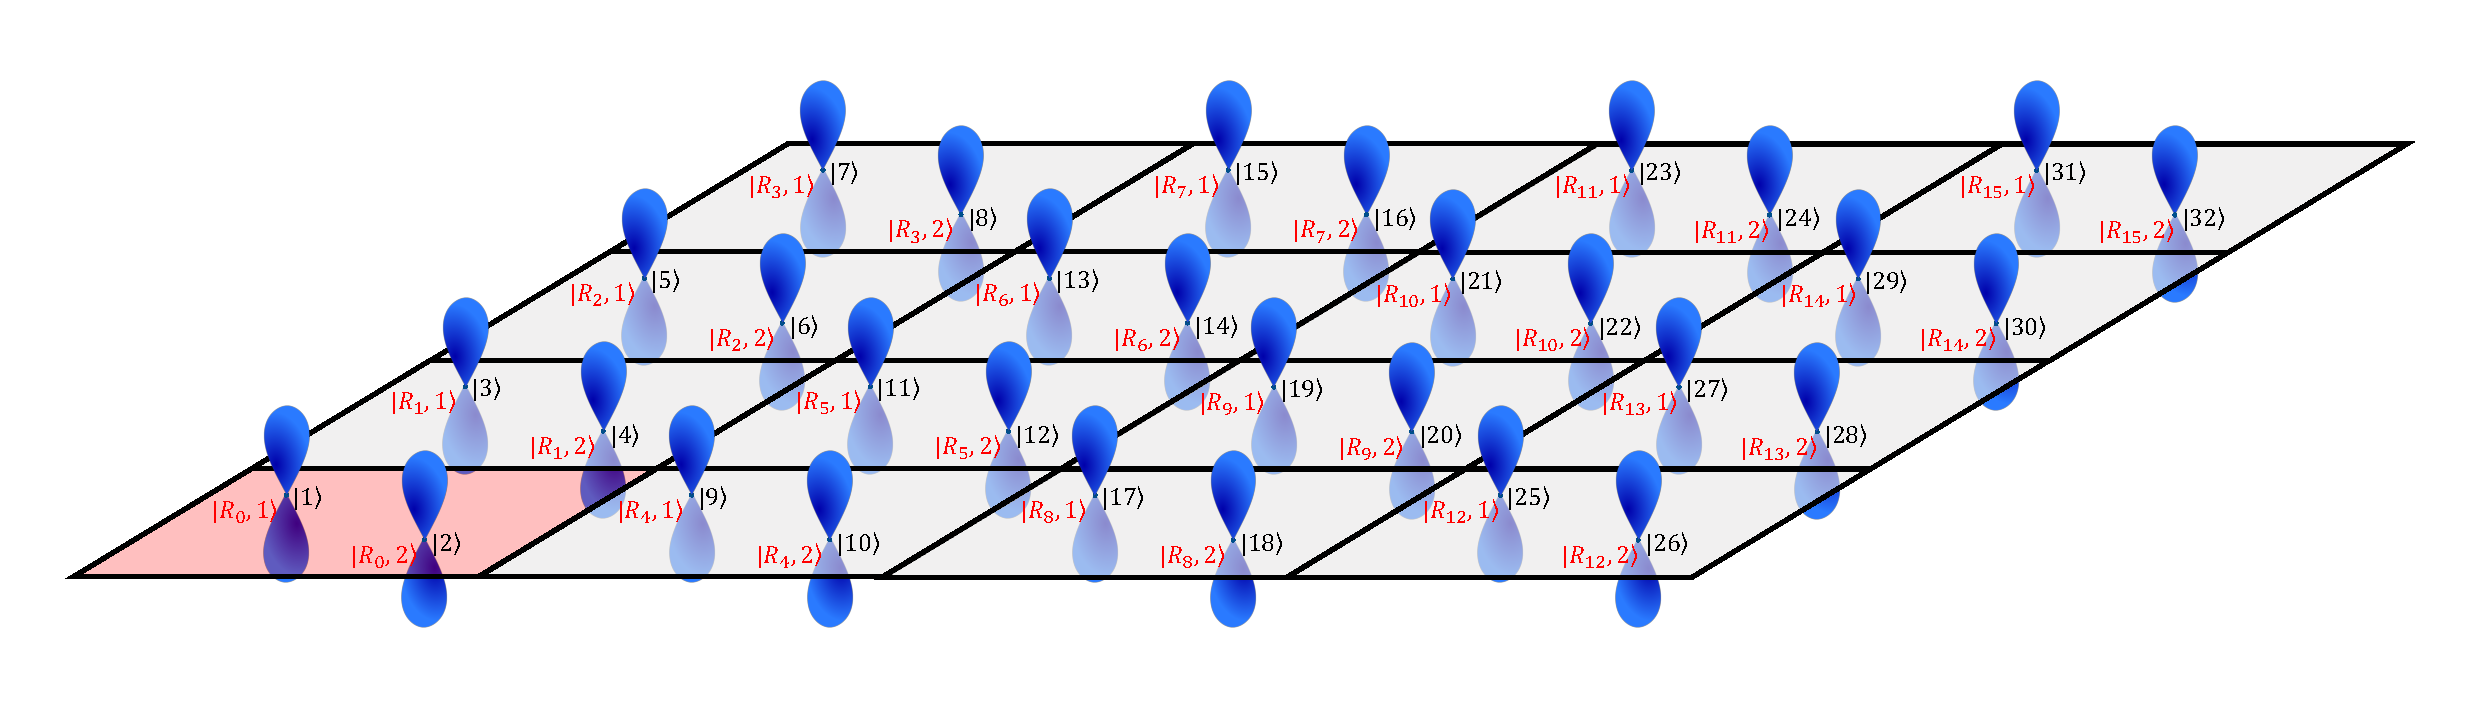
\includegraphics[width=\linewidth]{WF-pcell-scell.pdf}
    \caption[]{}
    \label{fig:map-wf}
\end{figure}


\subsection{Workflow\label{sec:workflow}}

\begin{figure}
    \centering
    \subfloat[]{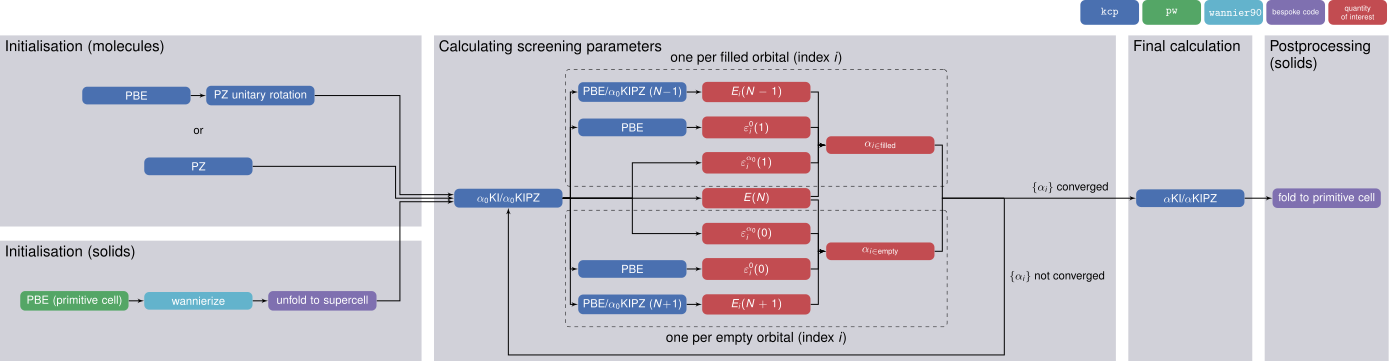
\includegraphics[width=\linewidth]{dscf_workflow.png}} \\
    \subfloat[]{
\includegraphics[width=\linewidth]{dfpt_workflow.png}}
    \caption[]{}
    \label{fig:workflow}
\end{figure}

\subsection{Computational details\label{sec:computational-details}}

\section{Results\label{sec:results-bands}}

